\section{Algorithm for near duplicate detection}
\label{section:luciv}
The improved version of the algorithm for duplicate detection from 
\cite{luciv2019interactive} is described in this chapter.
The main idea of the improvement is the utilization of the solution of the semi-local lcs problem.
First, we solve the semi-local lcs problem for the pattern against the entire text and then process a specific part of the string-substring submatrix of the solution.
We will emulate the first and the second phases of the original algorithm by doing this. The third phase remains the same.
Thus, we have improved the overall time complexity of the original algorithm and maintained its properties.


\subsection{Algorithm description}
Algorithm consists of three phases as the original one.
Algorithm pseudocode is presented in Algorithm~\ref{alg:patternMathing1}.

Note that in common case  the minimum edit score  can be expressed via maxmimal alignment score. The edit score from the original  algorithm expressed via alignment score with following weights:
\begin{equation}\label{weightAppr}
    (w_{+},w_{0},w_{-}) = (0,-2,-1)
\end{equation}
By virtue of formula (ref), the weights of the normalized scheme will be as follows:
\begin{equation}
    (0, -2, -1) \rightarrow (1,\frac{\mu=0}{v=1}, 0)
\end{equation}
Thereby, using normalization, the minimal edit score in the original algorithm can be reduced to \emph{semi-local lcs}. Given some lcs score, the associated minimal edit score can be obtained by first applying reverse regularization via (ref) and then adding a minus sign to the result.

Now we describe each phase in detail.

\textbf{First phase}. 
The first phase refers to solving semi-local problem for pattern $p$ against text $t$ (Line 1) and obtaining associated with it semi-local kernel $P^{str-sub}_{p,t}$ (Lines 2-3).
This kernel is an implicit presentation of string-substring matrix $M^{str-sub}_{p,t}$ that contains all lcs scores of pattern $p$ against all substrings of text $t$ (ref to theorem).
Further, for simplicity explanation, we will reason in terms of matrix $M^{str-sub}_{p,t}$.

\textbf{Second phase}.
At the second phase we process a text $t$ with a sliding window of size $\frac{|p|}{k}$ with a one symbol step  where $k  \in [\frac{1}{\sqrt{3}},1]$ is a similarity measure as in \cite{luciv2019interactive}.
Then within each window $w$, we process all substrings with sizes in the interval $I$ to find the substring that has the highest minimal edit score with pattern $p$. If there are several substrings within the considered window with the same minimal edit score, then the longest one will be taken.
We call such substrings a \emph{good} ones.
Moreover, to conform with the original algorithm, we leave only those substrings whose associated edit score of pattern $p$ against window $w$ is less than or equals to the defined threshold $k_{di}$\footnote{In the original algorithm, we first select suitable windows and then process them whereas in our approach we first process each window and only then select appropriate substrings within each window}.

The presence of matrix $M^{str-sub}_{p,t}$ allows us to process this phase asymptotically optimal.
First, all substrings with lengths in interval $I$ lie exactly in a diagonal slice (trapezoid in fig ) with width equals to $width:=\frac{|p|}{k} - |p|*k = |p|(\frac{1}{k}-k)$  in  $M^{str-sub}_{p,t}$.
The jagged triangles represent each window $w$ of text $t$ \footnote{ We also may consider square matrices but it superfluous because elements that lie below the main diagonal represents substrings with inappropriate small lengths}.
Thus, we only need to process cells in this diagonal during the second phase.

During the first traverse we query scores of each window $w$ against pattern $p$ and store them in list $L_{|w|}$. It is simply a one-way passage through diagonal\footnote{Cells $(i_{l},j_{l})$ whose indices satisfy the following equality: $j_{l}-i_{l} = \frac{|p|}{k}$} of size $O(|t|)$. This list will be needed further to leave only appropriate substrings within each window.

During the second traverse, we visit each cell that lies in the trapezoid associated with all substrings with lengths in interval $I$ in  the matrix $M^{str-sub}_{p,t}$.
The traversal algorithm for the second passage is shown in Fig.  ref {passage}.
We process diagonal in column fashion starting from the cell (0,$\frac{|p|}*k$).
As part of the traversal, we will maintain a  double linked list $rowMin$ that holds the following invariant at the end of processing some window $w$: 
$rowMin$ contains the largest substrings with the minimal edit score for the current suffixes of window $w$.
To find the  \emph{good} substring in current window $w$ we need to get the largest substring with the minimal edit score from $rowMin$. Then we will add this substring to $W_{2}$ if the associated window $w$ has the edit score less than or equals to $k_{di}$ (need just to check element of list $L_{|w|}$).
Then to get \emph{good} substring for the next window we remove the head of $rowMin$ and add a dummy element to the tail.
The first one represents a suffix which not fully contains in the current window,  the last one represents a new suffix that contains in the new window and now satisfies length constraints. 
After that, while processing the next column we update $rowMin$ and repeat the previous process. 

At the end of this phase, we have obtained a set $W_2$.

\textbf{Third phase}. 
This phase remains the same as in base algorithm.
 
\begin{figure}
	\centering
   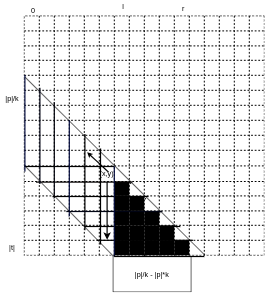
\includegraphics[width=0.4\columnwidth]{figures/M2.png}
   \caption{An example of processing matrix $M$.
   Here we goes from the end of the text. The width of diagonal is $\frac{|p|}{k} - |p|*k$.
Diagonal represent a set of substrings  of size in interval $I$ in text $t$.
Each triangular corresponds to sliding window in \cite{luciv2019interactive}.   
   }\label{M2}
\end{figure}




\begin{algorithm}[!t]
\caption{PATTERN BASED NEAR DUPLICATE
SEARCH ALGORITHM VIA SEMI-LOCAL SA}
\label{alg:patternMathing1}
Input: pattern $p$, text $t$, similiarity measure $k \in  ( \frac{1}{\sqrt{3}} ,1  ]$\\
Output: Set of non-intersected clones of pattern $p$ in text $t$
\begin{equation}
    k_{di}=|p|*(\frac{1}{k}+1)(1-k^2)
\end{equation}
\begin{equation}
 L_{w} = \frac{|p|} {k}
\end{equation}
\begin{equation}
  w = |p|(\frac{1}{k} - k)
\end{equation}
Pseudocode:
\begin{algorithmic}[1]
\STATE{$W = semilocalsa(p,t)$}
\COMMENT{1st phase}
\STATE{$H^{str-sub}_{p,t} = semilocalsa(p,t).stringSubstringMatrix$}
\STATE{$M[j,i] = -H^{str-sub}_{p,t}[i,j]  $}
\STATE{$lstW = queryWindows()$}
\COMMENT{2d phase}
\STATE{$W_2 = processDiagonal()$}
%% \STATE{$filter(W_2,k_{di})$}
\STATE{ $W_3 = UNIQUE(W_2)$}
\COMMENT{3rd phase unchanged}
\FOR{$w \in W_3$}
\IF{$\exists w^{'} \in W_3:w \subset w^{'} $}
\STATE{ $remove$ $w$ $from$ $W_3$}
\ENDIF
\ENDFOR
\RETURN $W_3$
\end{algorithmic}
\end{algorithm}

\begin{theorem}
Algorithm \ref{alg:patternMathing1} runs in $max(O(|t|*|p|),\ O(|t| * \log |t|))$ time with $O( |t| \log |t|)$ additional space where $p$ is pattern, $t$ is text, $|p| \leq |t|$, and $v=O(1)$ where $v$ is denominator of normalized mismatch score for semi-local sa $w_{normalized} = (1,\frac{\mu}{v},0)$.
\end{theorem}
\begin{proof}
  For each phases of algorithm we provide it's time and space bounds.
  
\emph{First phase.}
.. TODO
The time complexity of obtaining kernel $P_{p,t}$ is $O(|p|\times |t|)$ and requires $O(|t|+||)$ space.
The permutation matrix can be stored via two permutations of size $|t|$ for columns and rows.
It is simply two lists of size $|t|$.
Then, for random access query in specific position $(i,j)$ of matrix $H$ one need to check how many points are dominated by $H [i,j]$.
It can be done by checking all points of permutation matrix and requires $O(v * |t|)$ steps.
Thus, the total time and space complexity of the first phase are $O(v^2 *|p| * |t|)$ (time needed to solve semi-local sa) and $O(v*|t|)$ respectively.
Given $v=O(1)$ we have $O(|p| * |t|)$ and $O(|t|)$ respectively.

\emph{Second phase}.
For the sake of clarity, we omit $k$ factor in algorithm analysis since $k$ is just a constants within interval $(\frac{1}{\sqrt{3}},1]$.

%We proceed diagonal M as follows (\ref{M2}).
First, we query elements that lie in the diagonal that represent
substrings of size $L_{w}=\frac{|p|}{k}$ (to step onto $(0,|p|/k)$ cell we need to perform one orthogonal range query).
We denote them by $lstW$ (line 4).
Since we can use proposition~\ref{incremental} to access
adjacent elements 
the total complexity of this step is $O(|t|)$.
The total amount of querying cells is $O(|t|)$. 
Second, we again process matrix M.
More precisely, we process the diagonal of width $O(\frac{|p|}{k}-|p|*k)=O(|p|)$ that corresponds to all substrings with size in  $I=[|p|*k, \frac{|p|}{k}]$ interval (on Fig. \ref{M2} it is  trapezoid).
Note, that the bold triangle in Fig  \ref{M2} corresponds to the set of substrings with sizes in the interval $I$ that contains in the last substring with size $L_{w}$ of text $t$.
During processing each triangle we  additionally store list $longestForRow$ of size $\frac{|p|}{k}-|p|k$ that contains
for each row (represent prefix) the suffix that is most similar to pattern $p$ for given window (triangle on Fig. \ref{M2}).
This list updates every time when we shift triangle by one symbol step ($(x,y)\rightarrow (x-1,y-1)$).
Thus, to get the longest substring that most similar to pattern $p$ for the given window we simply need to check $longestForRow$. 
Thereby, we proceed as follows.
We check that the current window meets criteria
on similarity (it is just lookup to list $lstW$)
If so, then we find maximal substring among all associated with the current window (triangle) by checking $O(|p|)$ elements of $longestForRow$ and save it to set $W_{2}$ as described above (line 5).

Thus, the processing of each column of trapezia requires at most $O(|p|)$ time.
The total amount of columns is $(|t|)$.
Total time complexity of this phase is $O(|t|*|p|)$.
The space complexity of this phase is at most $O(|p|+|t|)=O(|t|)$.

\emph{Third phase}.
The third phase remains unchanged, thus have the same time and space bounds as in the base algorithm case.
Note, it possible to perform this phase in-place during the second phase which speedups the algorithm, i.e decreases space and time complexity to $O(|t|)$ and $O(|t|*|p|)$ respectively.
The third phase can be approximated as $O(|t| * log|t|)$ for both space and running time complexity.

Thus, the total alforithm running time is $max(O(t * p),\ O(t * \log t))$ while space complexity is $O(t * \log t)$.
\end{proof}

\begin{theorem}
Algorithm \ref{alg:patternMathing1} with scoring scheme $w = (0,-2,-1)$ preserves completnesses property of algorithm~\cite{luciv2019interactive} and has running time and space complexity $max(O(t*p),\ O(t* \log t))$ and $O(t *  \log t)$  respectively.
\end{theorem}

\begin{proof}
Edit distance in the base algorithm~\cite{luciv2019interactive} may be expressed as sequence alignment with following scoring scheme: 
$$w_{sa}=(w_{+},w_{0},w_{-}) = (0,-2,-1).$$

First, to get intial edit score we need to apply inverse operation:
$$editscore(a,b) = -sa(a,b,w_{sa}).$$
Next, $w_{sa}$ may be normalized using normalization~\ref{weightNormalization}:
$$(0, -2, -1) \rightarrow (1,\frac{\mu=0}{v=1}, 0).$$
Thus, $d_{di} \leq k_{di}$ is the same as $sa \geq -k_{di}$.

Second, let's carefull review phases 1 and 2 of given algorithms.
The base algorithm passes through the text with a sliding window to detect those fragments of size $L_{w}$ which have edit score above given threshold $k_{di}$.
Then within these fragments algorithm detects longest substrings that are most similar to pattern $p$ with size within interval $I=[pk,\ L_{w}]$.
The presented improved algorithm proceeds in a very similar way but, informally, phases are swapped.
First, it detects the longest substrings with size in interval $I$ for each window of the text.
Then, it proceeds in such way that for each window of size $L_{w}$ that has alignment score with pattern $p$ above given threshold $-k_{di}$  the longest substring most similar to $p$ is detected.
Thus, the results of the second phases of the algorithms are equal.
%Due to \todo{formula~\ref{editsa}} results of the second phases %of the algorithms are equal.
The third phase remains unchaned in the presented algorithm.
%% Thus, the presented algorithm preserves completeness.
Thus, the presented algorithm is complete.
For $w = (0,-2,-1)$, $v=1$ and algorithm running time and space complexity are as claimed.
%% For given $w = (0,-2,-1)$ we have $v=1$ then wehave running time as claimed.
\end{proof}

%At first algorithm \ref{luciv} pass through text $t$ with sliding window to detect those fragments which has similarity abobe given threhsold $k_{di}$ with size $\frac{p}{k}$.
%Then within these fragments algorithm detects longest suffixes most similar to pattern $p$ with size within  $pk...\frac{p}{k}$ interval.
%That how $A_1$ constucted.
%
%T%he second algorithm \ref{alg:patternMathing1} proceed in similar way but it first .
 .
%$Then filtering is perfomed in that way that only$
%That how $A_1$ constucted.
%those lonh suffices  left 
 %for those windows of size $\frac{p}{k}$ the longest suffix is left.

%T%%hus, $A_1=A_2$  by resulting equivalence of construction. 


